\documentclass[,man,floatsintext]{apa6}
\usepackage{lmodern}
\usepackage{amssymb,amsmath}
\usepackage{ifxetex,ifluatex}
\usepackage{fixltx2e} % provides \textsubscript
\ifnum 0\ifxetex 1\fi\ifluatex 1\fi=0 % if pdftex
  \usepackage[T1]{fontenc}
  \usepackage[utf8]{inputenc}
\else % if luatex or xelatex
  \ifxetex
    \usepackage{mathspec}
  \else
    \usepackage{fontspec}
  \fi
  \defaultfontfeatures{Ligatures=TeX,Scale=MatchLowercase}
\fi
% use upquote if available, for straight quotes in verbatim environments
\IfFileExists{upquote.sty}{\usepackage{upquote}}{}
% use microtype if available
\IfFileExists{microtype.sty}{%
\usepackage{microtype}
\UseMicrotypeSet[protrusion]{basicmath} % disable protrusion for tt fonts
}{}
\usepackage{hyperref}
\hypersetup{unicode=true,
            pdftitle={Supplemental materials: Instance theory predicts information theory: Episodic uncertainty as a determinant of keystroke dynamics},
            pdfauthor={Matthew J. C. Crump, Walter Lai, \& Nicholaus P. Brosowsky},
            pdfborder={0 0 0},
            breaklinks=true}
\urlstyle{same}  % don't use monospace font for urls
\usepackage{color}
\usepackage{fancyvrb}
\newcommand{\VerbBar}{|}
\newcommand{\VERB}{\Verb[commandchars=\\\{\}]}
\DefineVerbatimEnvironment{Highlighting}{Verbatim}{commandchars=\\\{\}}
% Add ',fontsize=\small' for more characters per line
\usepackage{framed}
\definecolor{shadecolor}{RGB}{248,248,248}
\newenvironment{Shaded}{\begin{snugshade}}{\end{snugshade}}
\newcommand{\AlertTok}[1]{\textcolor[rgb]{0.94,0.16,0.16}{#1}}
\newcommand{\AnnotationTok}[1]{\textcolor[rgb]{0.56,0.35,0.01}{\textbf{\textit{#1}}}}
\newcommand{\AttributeTok}[1]{\textcolor[rgb]{0.77,0.63,0.00}{#1}}
\newcommand{\BaseNTok}[1]{\textcolor[rgb]{0.00,0.00,0.81}{#1}}
\newcommand{\BuiltInTok}[1]{#1}
\newcommand{\CharTok}[1]{\textcolor[rgb]{0.31,0.60,0.02}{#1}}
\newcommand{\CommentTok}[1]{\textcolor[rgb]{0.56,0.35,0.01}{\textit{#1}}}
\newcommand{\CommentVarTok}[1]{\textcolor[rgb]{0.56,0.35,0.01}{\textbf{\textit{#1}}}}
\newcommand{\ConstantTok}[1]{\textcolor[rgb]{0.00,0.00,0.00}{#1}}
\newcommand{\ControlFlowTok}[1]{\textcolor[rgb]{0.13,0.29,0.53}{\textbf{#1}}}
\newcommand{\DataTypeTok}[1]{\textcolor[rgb]{0.13,0.29,0.53}{#1}}
\newcommand{\DecValTok}[1]{\textcolor[rgb]{0.00,0.00,0.81}{#1}}
\newcommand{\DocumentationTok}[1]{\textcolor[rgb]{0.56,0.35,0.01}{\textbf{\textit{#1}}}}
\newcommand{\ErrorTok}[1]{\textcolor[rgb]{0.64,0.00,0.00}{\textbf{#1}}}
\newcommand{\ExtensionTok}[1]{#1}
\newcommand{\FloatTok}[1]{\textcolor[rgb]{0.00,0.00,0.81}{#1}}
\newcommand{\FunctionTok}[1]{\textcolor[rgb]{0.00,0.00,0.00}{#1}}
\newcommand{\ImportTok}[1]{#1}
\newcommand{\InformationTok}[1]{\textcolor[rgb]{0.56,0.35,0.01}{\textbf{\textit{#1}}}}
\newcommand{\KeywordTok}[1]{\textcolor[rgb]{0.13,0.29,0.53}{\textbf{#1}}}
\newcommand{\NormalTok}[1]{#1}
\newcommand{\OperatorTok}[1]{\textcolor[rgb]{0.81,0.36,0.00}{\textbf{#1}}}
\newcommand{\OtherTok}[1]{\textcolor[rgb]{0.56,0.35,0.01}{#1}}
\newcommand{\PreprocessorTok}[1]{\textcolor[rgb]{0.56,0.35,0.01}{\textit{#1}}}
\newcommand{\RegionMarkerTok}[1]{#1}
\newcommand{\SpecialCharTok}[1]{\textcolor[rgb]{0.00,0.00,0.00}{#1}}
\newcommand{\SpecialStringTok}[1]{\textcolor[rgb]{0.31,0.60,0.02}{#1}}
\newcommand{\StringTok}[1]{\textcolor[rgb]{0.31,0.60,0.02}{#1}}
\newcommand{\VariableTok}[1]{\textcolor[rgb]{0.00,0.00,0.00}{#1}}
\newcommand{\VerbatimStringTok}[1]{\textcolor[rgb]{0.31,0.60,0.02}{#1}}
\newcommand{\WarningTok}[1]{\textcolor[rgb]{0.56,0.35,0.01}{\textbf{\textit{#1}}}}
\usepackage{graphicx,grffile}
\makeatletter
\def\maxwidth{\ifdim\Gin@nat@width>\linewidth\linewidth\else\Gin@nat@width\fi}
\def\maxheight{\ifdim\Gin@nat@height>\textheight\textheight\else\Gin@nat@height\fi}
\makeatother
% Scale images if necessary, so that they will not overflow the page
% margins by default, and it is still possible to overwrite the defaults
% using explicit options in \includegraphics[width, height, ...]{}
\setkeys{Gin}{width=\maxwidth,height=\maxheight,keepaspectratio}
\IfFileExists{parskip.sty}{%
\usepackage{parskip}
}{% else
\setlength{\parindent}{0pt}
\setlength{\parskip}{6pt plus 2pt minus 1pt}
}
\setlength{\emergencystretch}{3em}  % prevent overfull lines
\providecommand{\tightlist}{%
  \setlength{\itemsep}{0pt}\setlength{\parskip}{0pt}}
\setcounter{secnumdepth}{0}
% Redefines (sub)paragraphs to behave more like sections
\ifx\paragraph\undefined\else
\let\oldparagraph\paragraph
\renewcommand{\paragraph}[1]{\oldparagraph{#1}\mbox{}}
\fi
\ifx\subparagraph\undefined\else
\let\oldsubparagraph\subparagraph
\renewcommand{\subparagraph}[1]{\oldsubparagraph{#1}\mbox{}}
\fi

%%% Use protect on footnotes to avoid problems with footnotes in titles
\let\rmarkdownfootnote\footnote%
\def\footnote{\protect\rmarkdownfootnote}


  \title{Supplemental materials: Instance theory predicts information theory: Episodic uncertainty as a determinant of keystroke dynamics}
    \author{Matthew J. C. Crump\textsuperscript{1,2}, Walter Lai\textsuperscript{1}, \& Nicholaus P. Brosowsky\textsuperscript{2}}
    \date{}
  
\shorttitle{Supplemental materials}
\affiliation{
\vspace{0.5cm}
\textsuperscript{1} Brooklyn College of the City University of New York\\\textsuperscript{2} The Graduate Center of the City University of New York}
\keywords{\newline\indent Word count: }
\usepackage{csquotes}
\usepackage{upgreek}
\captionsetup{font=singlespacing,justification=justified}

\usepackage{longtable}
\usepackage{lscape}
\usepackage{multirow}
\usepackage{tabularx}
\usepackage[flushleft]{threeparttable}
\usepackage{threeparttablex}

\newenvironment{lltable}{\begin{landscape}\begin{center}\begin{ThreePartTable}}{\end{ThreePartTable}\end{center}\end{landscape}}

\makeatletter
\newcommand\LastLTentrywidth{1em}
\newlength\longtablewidth
\setlength{\longtablewidth}{1in}
\newcommand{\getlongtablewidth}{\begingroup \ifcsname LT@\roman{LT@tables}\endcsname \global\longtablewidth=0pt \renewcommand{\LT@entry}[2]{\global\advance\longtablewidth by ##2\relax\gdef\LastLTentrywidth{##2}}\@nameuse{LT@\roman{LT@tables}} \fi \endgroup}
\setlength{\parskip}{0.25cm plus4mm minus3mm}

\authornote{In addition to these supplemental materials, all of the data and analysis scripts are available at \url{https://osf.io/bdnqr/} (Crump, Lai, \& Brosowsky, 2018). This work was supported by a grant from NSF (1353360) to Matthew Crump.

Correspondence concerning this article should be addressed to Matthew J. C. Crump, Brooklyn College of CUNY, 2900 Bedford Avenue, Brooklyn, NY, 11210. E-mail: \href{mailto:mcrump@brooklyn.cuny.edu}{\nolinkurl{mcrump@brooklyn.cuny.edu}}}

\abstract{
This .pdf contains supplemental materials.


}

\begin{document}
\maketitle

\hypertarget{expanded-description-of-methods}{%
\section{Expanded description of Methods}\label{expanded-description-of-methods}}

\hypertarget{participants}{%
\subsection{Participants}\label{participants}}

400 participants were recruited from Amazon's mechanical turk (restricted to people from the USA, with over 90\% completion rate). Data were only analyzed for the 346 participants who successfully completed the task (98 men, 237 women, 11 no response). Additional demographic information is reported in Behmer and Crump (2017). The procedure was approved by the institutional review board at Brooklyn College of the City University of New York.

\hypertarget{stimuli-and-apparatus}{%
\subsection{Stimuli and Apparatus}\label{stimuli-and-apparatus}}

From Behmer and Crump (2017), \enquote{Typists copy-typed five normal paragraphs from the Simple English Wiki, a version of the online encyclopedia Wikipedia written in basic English. Four of the paragraphs were from the entry about cats (\url{http://simple.wikipedia}. org/wiki/Cat), and one paragraph was from the entry for music (\url{http://simple.wikipedia.org/wiki/Music}). Each normal paragraph had an average of 131 words (range 124--137).} In addition to typing English paragraphs, each typist also copy typed a paragraph of 5 letter random strings, and a paragraph of 5 letter strings that approximated the bigram structure of English.

The apparatus was a website displaying a textbox containing a single paragraph. Paragraph text was black, presented in 14 pt, Helvetica font. JavaScript was used to record keystroke timestamps in milliseconds.

\hypertarget{design-and-procedure}{%
\subsection{Design and Procedure}\label{design-and-procedure}}

From Behmer and Crump (2017), \enquote{Participants were instructed to begin typing with the first letter in the paragraph. Correctly typed letters turned green, and typists could only proceed to the next by typing the current letter correctly. After completing the task, participants were presented with a debriefing, and a form to provide any feedback about the task. The task took around 30 to 45 minutes to complete. Participants who completed the task were paid \$1.}

\hypertarget{code-for-reproducing-instance-theory-simulation-of-hyman-1953}{%
\section{Code for reproducing instance theory simulation of Hyman (1953)}\label{code-for-reproducing-instance-theory-simulation-of-hyman-1953}}

\begin{Shaded}
\begin{Highlighting}[]
\NormalTok{hyman <-}\StringTok{ }\KeywordTok{list}\NormalTok{(}
  \DataTypeTok{e1_1 =} \KeywordTok{list}\NormalTok{(}\DataTypeTok{stims =} \DecValTok{1}\NormalTok{,}
              \DataTypeTok{probs =} \DecValTok{1}\NormalTok{),}
  \DataTypeTok{e1_2 =} \KeywordTok{list}\NormalTok{(}\DataTypeTok{stims =} \DecValTok{1}\OperatorTok{:}\DecValTok{2}\NormalTok{,}
              \DataTypeTok{probs =} \KeywordTok{rep}\NormalTok{(}\DecValTok{1}\OperatorTok{/}\DecValTok{2}\NormalTok{,}\DecValTok{2}\NormalTok{)),}
  \DataTypeTok{e1_3 =} \KeywordTok{list}\NormalTok{(}\DataTypeTok{stims =} \DecValTok{1}\OperatorTok{:}\DecValTok{3}\NormalTok{,}
              \DataTypeTok{probs =} \KeywordTok{rep}\NormalTok{(}\DecValTok{1}\OperatorTok{/}\DecValTok{3}\NormalTok{,}\DecValTok{3}\NormalTok{)),}
  \DataTypeTok{e1_4 =} \KeywordTok{list}\NormalTok{(}\DataTypeTok{stims =} \DecValTok{1}\OperatorTok{:}\DecValTok{4}\NormalTok{,}
              \DataTypeTok{probs =} \KeywordTok{rep}\NormalTok{(}\DecValTok{1}\OperatorTok{/}\DecValTok{4}\NormalTok{,}\DecValTok{4}\NormalTok{)),}
  \DataTypeTok{e1_5 =} \KeywordTok{list}\NormalTok{(}\DataTypeTok{stims =} \DecValTok{1}\OperatorTok{:}\DecValTok{5}\NormalTok{,}
              \DataTypeTok{probs =} \KeywordTok{rep}\NormalTok{(}\DecValTok{1}\OperatorTok{/}\DecValTok{5}\NormalTok{,}\DecValTok{5}\NormalTok{)),}
  \DataTypeTok{e1_6 =} \KeywordTok{list}\NormalTok{(}\DataTypeTok{stims =} \DecValTok{1}\OperatorTok{:}\DecValTok{6}\NormalTok{,}
              \DataTypeTok{probs =} \KeywordTok{rep}\NormalTok{(}\DecValTok{1}\OperatorTok{/}\DecValTok{6}\NormalTok{,}\DecValTok{6}\NormalTok{)),}
  \DataTypeTok{e1_7 =} \KeywordTok{list}\NormalTok{(}\DataTypeTok{stims =} \DecValTok{1}\OperatorTok{:}\DecValTok{7}\NormalTok{,}
              \DataTypeTok{probs =} \KeywordTok{rep}\NormalTok{(}\DecValTok{1}\OperatorTok{/}\DecValTok{7}\NormalTok{,}\DecValTok{7}\NormalTok{)),}
  \DataTypeTok{e1_8 =} \KeywordTok{list}\NormalTok{(}\DataTypeTok{stims =} \DecValTok{1}\OperatorTok{:}\DecValTok{8}\NormalTok{,}
              \DataTypeTok{probs =} \KeywordTok{rep}\NormalTok{(}\DecValTok{1}\OperatorTok{/}\DecValTok{8}\NormalTok{,}\DecValTok{8}\NormalTok{)),}
  \DataTypeTok{e2_1 =} \KeywordTok{list}\NormalTok{(}\DataTypeTok{stims =} \DecValTok{1}\OperatorTok{:}\DecValTok{2}\NormalTok{,}
              \DataTypeTok{probs =} \KeywordTok{c}\NormalTok{(}\DecValTok{9}\OperatorTok{/}\DecValTok{10}\NormalTok{,}\DecValTok{1}\OperatorTok{/}\DecValTok{10}\NormalTok{)),}
  \DataTypeTok{e2_2 =} \KeywordTok{list}\NormalTok{(}\DataTypeTok{stims =} \DecValTok{1}\OperatorTok{:}\DecValTok{2}\NormalTok{,}
              \DataTypeTok{probs =} \KeywordTok{c}\NormalTok{(}\DecValTok{8}\OperatorTok{/}\DecValTok{10}\NormalTok{,}\DecValTok{2}\OperatorTok{/}\DecValTok{10}\NormalTok{)),}
  \DataTypeTok{e2_3 =} \KeywordTok{list}\NormalTok{(}\DataTypeTok{stims =} \DecValTok{1}\OperatorTok{:}\DecValTok{4}\NormalTok{,}
              \DataTypeTok{probs =} \KeywordTok{c}\NormalTok{(}\DecValTok{13}\OperatorTok{/}\DecValTok{16}\NormalTok{,}\KeywordTok{rep}\NormalTok{(}\DecValTok{1}\OperatorTok{/}\DecValTok{16}\NormalTok{,}\DecValTok{3}\NormalTok{))),}
  \DataTypeTok{e2_4 =} \KeywordTok{list}\NormalTok{(}\DataTypeTok{stims =} \DecValTok{1}\OperatorTok{:}\DecValTok{6}\NormalTok{,}
              \DataTypeTok{probs =} \KeywordTok{c}\NormalTok{(}\DecValTok{15}\OperatorTok{/}\DecValTok{20}\NormalTok{,}\KeywordTok{rep}\NormalTok{(}\DecValTok{1}\OperatorTok{/}\DecValTok{20}\NormalTok{,}\DecValTok{5}\NormalTok{))),}
  \DataTypeTok{e2_5 =} \KeywordTok{list}\NormalTok{(}\DataTypeTok{stims =} \DecValTok{1}\OperatorTok{:}\DecValTok{4}\NormalTok{,}
              \DataTypeTok{probs =} \KeywordTok{c}\NormalTok{(}\DecValTok{4}\OperatorTok{/}\DecValTok{8}\NormalTok{,}\DecValTok{2}\OperatorTok{/}\DecValTok{8}\NormalTok{,}\KeywordTok{rep}\NormalTok{(}\DecValTok{1}\OperatorTok{/}\DecValTok{8}\NormalTok{,}\DecValTok{2}\NormalTok{))),}
  \DataTypeTok{e2_6 =} \KeywordTok{list}\NormalTok{(}\DataTypeTok{stims =} \DecValTok{1}\OperatorTok{:}\DecValTok{6}\NormalTok{,}
              \DataTypeTok{probs =} \KeywordTok{c}\NormalTok{(}\DecValTok{5}\OperatorTok{/}\DecValTok{10}\NormalTok{,}\KeywordTok{rep}\NormalTok{(}\DecValTok{1}\OperatorTok{/}\DecValTok{10}\NormalTok{,}\DecValTok{5}\NormalTok{))),}
  \DataTypeTok{e2_7 =} \KeywordTok{list}\NormalTok{(}\DataTypeTok{stims =} \DecValTok{1}\OperatorTok{:}\DecValTok{8}\NormalTok{,}
              \DataTypeTok{probs =} \KeywordTok{c}\NormalTok{(}\DecValTok{8}\OperatorTok{/}\DecValTok{16}\NormalTok{,}\DecValTok{2}\OperatorTok{/}\DecValTok{16}\NormalTok{,}\KeywordTok{rep}\NormalTok{(}\DecValTok{1}\OperatorTok{/}\DecValTok{16}\NormalTok{,}\DecValTok{6}\NormalTok{))),}
  \DataTypeTok{e2_8 =} \KeywordTok{list}\NormalTok{(}\DataTypeTok{stims =} \DecValTok{1}\OperatorTok{:}\DecValTok{8}\NormalTok{,}
              \DataTypeTok{probs =} \KeywordTok{c}\NormalTok{(}\KeywordTok{rep}\NormalTok{(}\DecValTok{4}\OperatorTok{/}\DecValTok{16}\NormalTok{,}\DecValTok{2}\NormalTok{),}\KeywordTok{rep}\NormalTok{(}\DecValTok{2}\OperatorTok{/}\DecValTok{16}\NormalTok{,}\DecValTok{2}\NormalTok{),}\KeywordTok{rep}\NormalTok{(}\DecValTok{1}\OperatorTok{/}\DecValTok{16}\NormalTok{,}\DecValTok{4}\NormalTok{))),}
  \DataTypeTok{e3_1 =} \KeywordTok{list}\NormalTok{(}\DataTypeTok{stims =} \KeywordTok{c}\NormalTok{(}\DecValTok{11}\NormalTok{,}\DecValTok{12}\NormalTok{,}\DecValTok{21}\NormalTok{,}\DecValTok{22}\NormalTok{),}
              \DataTypeTok{probs =} \KeywordTok{c}\NormalTok{(}\DecValTok{2}\OperatorTok{/}\DecValTok{10}\NormalTok{,}\DecValTok{8}\OperatorTok{/}\DecValTok{10}\NormalTok{,}\DecValTok{0}\NormalTok{,}\DecValTok{0}\NormalTok{)),}
  \DataTypeTok{e3_2 =} \KeywordTok{list}\NormalTok{(}\DataTypeTok{stims =} \KeywordTok{c}\NormalTok{(}\DecValTok{11}\NormalTok{,}\DecValTok{12}\NormalTok{,}\DecValTok{13}\NormalTok{,}
                        \DecValTok{21}\NormalTok{,}\DecValTok{22}\NormalTok{,}\DecValTok{23}\NormalTok{,}
                        \DecValTok{31}\NormalTok{,}\DecValTok{32}\NormalTok{,}\DecValTok{33}\NormalTok{),}
              \DataTypeTok{probs =} \KeywordTok{c}\NormalTok{(}\DecValTok{1}\OperatorTok{/}\DecValTok{10}\NormalTok{,}\DecValTok{8}\OperatorTok{/}\DecValTok{10}\NormalTok{,}\DecValTok{1}\OperatorTok{/}\DecValTok{10}\NormalTok{,}
                        \DecValTok{0}\NormalTok{,}\DecValTok{0}\NormalTok{,}\DecValTok{0}\NormalTok{,}
                        \DecValTok{0}\NormalTok{,}\DecValTok{0}\NormalTok{,}\DecValTok{0}\NormalTok{)),}
  \DataTypeTok{e3_3 =}  \KeywordTok{list}\NormalTok{(}\DataTypeTok{stims =} \KeywordTok{c}\NormalTok{(}\DecValTok{11}\NormalTok{,}\DecValTok{12}\NormalTok{,}\DecValTok{13}\NormalTok{,}\DecValTok{14}\NormalTok{,}
                         \DecValTok{21}\NormalTok{,}\DecValTok{22}\NormalTok{,}\DecValTok{23}\NormalTok{,}\DecValTok{24}\NormalTok{,}
                         \DecValTok{31}\NormalTok{,}\DecValTok{32}\NormalTok{,}\DecValTok{33}\NormalTok{,}\DecValTok{34}\NormalTok{),}
               \DataTypeTok{probs =} \KeywordTok{c}\NormalTok{(}\DecValTok{7}\OperatorTok{/}\DecValTok{10}\NormalTok{,}\DecValTok{1}\OperatorTok{/}\DecValTok{10}\NormalTok{,}\DecValTok{1}\OperatorTok{/}\DecValTok{10}\NormalTok{,}\DecValTok{1}\OperatorTok{/}\DecValTok{10}\NormalTok{,}
                         \DecValTok{0}\NormalTok{,}\DecValTok{0}\NormalTok{,}\DecValTok{0}\NormalTok{,}\DecValTok{0}\NormalTok{,}
                         \DecValTok{0}\NormalTok{,}\DecValTok{0}\NormalTok{,}\DecValTok{0}\NormalTok{,}\DecValTok{0}\NormalTok{,}
                         \DecValTok{0}\NormalTok{,}\DecValTok{0}\NormalTok{,}\DecValTok{0}\NormalTok{,}\DecValTok{0}\NormalTok{)),}
  \DataTypeTok{e3_4 =}  \KeywordTok{list}\NormalTok{(}\DataTypeTok{stims =} \KeywordTok{c}\NormalTok{(}\DecValTok{11}\NormalTok{,}\DecValTok{12}\NormalTok{,}\DecValTok{13}\NormalTok{,}\DecValTok{14}\NormalTok{,}
                         \DecValTok{21}\NormalTok{,}\DecValTok{22}\NormalTok{,}\DecValTok{23}\NormalTok{,}\DecValTok{24}\NormalTok{,}
                         \DecValTok{31}\NormalTok{,}\DecValTok{32}\NormalTok{,}\DecValTok{33}\NormalTok{,}\DecValTok{34}\NormalTok{),}
               \DataTypeTok{probs =} \KeywordTok{c}\NormalTok{(}\DecValTok{1}\OperatorTok{/}\DecValTok{6}\NormalTok{,}\DecValTok{3}\OperatorTok{/}\DecValTok{6}\NormalTok{,}\DecValTok{1}\OperatorTok{/}\DecValTok{6}\NormalTok{,}\DecValTok{1}\OperatorTok{/}\DecValTok{6}\NormalTok{,}
                         \DecValTok{0}\NormalTok{,}\DecValTok{0}\NormalTok{,}\DecValTok{0}\NormalTok{,}\DecValTok{0}\NormalTok{,}
                         \DecValTok{0}\NormalTok{,}\DecValTok{0}\NormalTok{,}\DecValTok{0}\NormalTok{,}\DecValTok{0}\NormalTok{,}
                         \DecValTok{0}\NormalTok{,}\DecValTok{0}\NormalTok{,}\DecValTok{0}\NormalTok{,}\DecValTok{0}\NormalTok{)),}
  \DataTypeTok{e3_5 =}  \KeywordTok{list}\NormalTok{(}\DataTypeTok{stims =} \KeywordTok{c}\NormalTok{(}\DecValTok{11}\NormalTok{,}\DecValTok{12}\NormalTok{,}\DecValTok{13}\NormalTok{,}\DecValTok{14}\NormalTok{,}\DecValTok{15}\NormalTok{,}\DecValTok{16}\NormalTok{,}\DecValTok{17}\NormalTok{,}\DecValTok{18}\NormalTok{,}
                         \DecValTok{21}\NormalTok{,}\DecValTok{22}\NormalTok{,}\DecValTok{23}\NormalTok{,}\DecValTok{24}\NormalTok{,}\DecValTok{25}\NormalTok{,}\DecValTok{26}\NormalTok{,}\DecValTok{27}\NormalTok{,}\DecValTok{28}\NormalTok{,}
                         \DecValTok{31}\NormalTok{,}\DecValTok{32}\NormalTok{,}\DecValTok{33}\NormalTok{,}\DecValTok{34}\NormalTok{,}\DecValTok{35}\NormalTok{,}\DecValTok{36}\NormalTok{,}\DecValTok{37}\NormalTok{,}\DecValTok{38}\NormalTok{,}
                         \DecValTok{41}\NormalTok{,}\DecValTok{42}\NormalTok{,}\DecValTok{43}\NormalTok{,}\DecValTok{44}\NormalTok{,}\DecValTok{45}\NormalTok{,}\DecValTok{46}\NormalTok{,}\DecValTok{47}\NormalTok{,}\DecValTok{48}\NormalTok{,}
                         \DecValTok{51}\NormalTok{,}\DecValTok{52}\NormalTok{,}\DecValTok{53}\NormalTok{,}\DecValTok{54}\NormalTok{,}\DecValTok{55}\NormalTok{,}\DecValTok{56}\NormalTok{,}\DecValTok{57}\NormalTok{,}\DecValTok{58}\NormalTok{,}
                         \DecValTok{61}\NormalTok{,}\DecValTok{62}\NormalTok{,}\DecValTok{63}\NormalTok{,}\DecValTok{64}\NormalTok{,}\DecValTok{65}\NormalTok{,}\DecValTok{66}\NormalTok{,}\DecValTok{67}\NormalTok{,}\DecValTok{68}\NormalTok{,}
                         \DecValTok{71}\NormalTok{,}\DecValTok{72}\NormalTok{,}\DecValTok{73}\NormalTok{,}\DecValTok{74}\NormalTok{,}\DecValTok{75}\NormalTok{,}\DecValTok{76}\NormalTok{,}\DecValTok{77}\NormalTok{,}\DecValTok{78}\NormalTok{,}
                         \DecValTok{81}\NormalTok{,}\DecValTok{82}\NormalTok{,}\DecValTok{83}\NormalTok{,}\DecValTok{84}\NormalTok{,}\DecValTok{85}\NormalTok{,}\DecValTok{86}\NormalTok{,}\DecValTok{87}\NormalTok{,}\DecValTok{88}\NormalTok{),}
               \DataTypeTok{probs =} \KeywordTok{c}\NormalTok{(}\DecValTok{1}\OperatorTok{/}\DecValTok{16}\NormalTok{,}\DecValTok{9}\OperatorTok{/}\DecValTok{16}\NormalTok{,}\DecValTok{1}\OperatorTok{/}\DecValTok{16}\NormalTok{,}\DecValTok{1}\OperatorTok{/}\DecValTok{16}\NormalTok{,}\DecValTok{1}\OperatorTok{/}\DecValTok{16}\NormalTok{,}\DecValTok{1}\OperatorTok{/}\DecValTok{16}\NormalTok{,}\DecValTok{1}\OperatorTok{/}\DecValTok{16}\NormalTok{,}\DecValTok{1}\OperatorTok{/}\DecValTok{16}\NormalTok{,}
                         \DecValTok{0}\NormalTok{,}\DecValTok{0}\NormalTok{,}\DecValTok{0}\NormalTok{,}\DecValTok{0}\NormalTok{,}\DecValTok{0}\NormalTok{,}\DecValTok{0}\NormalTok{,}\DecValTok{0}\NormalTok{,}\DecValTok{0}\NormalTok{,}
                         \DecValTok{0}\NormalTok{,}\DecValTok{0}\NormalTok{,}\DecValTok{0}\NormalTok{,}\DecValTok{0}\NormalTok{,}\DecValTok{0}\NormalTok{,}\DecValTok{0}\NormalTok{,}\DecValTok{0}\NormalTok{,}\DecValTok{0}\NormalTok{,}
                         \DecValTok{0}\NormalTok{,}\DecValTok{0}\NormalTok{,}\DecValTok{0}\NormalTok{,}\DecValTok{0}\NormalTok{,}\DecValTok{0}\NormalTok{,}\DecValTok{0}\NormalTok{,}\DecValTok{0}\NormalTok{,}\DecValTok{0}\NormalTok{,}
                         \DecValTok{0}\NormalTok{,}\DecValTok{0}\NormalTok{,}\DecValTok{0}\NormalTok{,}\DecValTok{0}\NormalTok{,}\DecValTok{0}\NormalTok{,}\DecValTok{0}\NormalTok{,}\DecValTok{0}\NormalTok{,}\DecValTok{0}\NormalTok{,}
                         \DecValTok{0}\NormalTok{,}\DecValTok{0}\NormalTok{,}\DecValTok{0}\NormalTok{,}\DecValTok{0}\NormalTok{,}\DecValTok{0}\NormalTok{,}\DecValTok{0}\NormalTok{,}\DecValTok{0}\NormalTok{,}\DecValTok{0}\NormalTok{,}
                         \DecValTok{0}\NormalTok{,}\DecValTok{0}\NormalTok{,}\DecValTok{0}\NormalTok{,}\DecValTok{0}\NormalTok{,}\DecValTok{0}\NormalTok{,}\DecValTok{0}\NormalTok{,}\DecValTok{0}\NormalTok{,}\DecValTok{0}\NormalTok{,}
                         \DecValTok{0}\NormalTok{,}\DecValTok{0}\NormalTok{,}\DecValTok{0}\NormalTok{,}\DecValTok{0}\NormalTok{,}\DecValTok{0}\NormalTok{,}\DecValTok{0}\NormalTok{,}\DecValTok{0}\NormalTok{,}\DecValTok{0}\NormalTok{)),}
  \DataTypeTok{e3_6 =} \KeywordTok{list}\NormalTok{(}\DataTypeTok{stims =} \KeywordTok{c}\NormalTok{(}\DecValTok{11}\NormalTok{,}\DecValTok{12}\NormalTok{,}\DecValTok{13}\NormalTok{,}
                        \DecValTok{21}\NormalTok{,}\DecValTok{22}\NormalTok{,}\DecValTok{23}\NormalTok{,}
                        \DecValTok{31}\NormalTok{,}\DecValTok{32}\NormalTok{,}\DecValTok{33}\NormalTok{),}
              \DataTypeTok{probs =} \KeywordTok{c}\NormalTok{(}\DecValTok{0}\NormalTok{,}\DecValTok{1}\OperatorTok{/}\DecValTok{2}\NormalTok{,}\DecValTok{1}\OperatorTok{/}\DecValTok{2}\NormalTok{,}
                        \DecValTok{0}\NormalTok{,}\DecValTok{0}\NormalTok{,}\DecValTok{0}\NormalTok{,}
                        \DecValTok{0}\NormalTok{,}\DecValTok{0}\NormalTok{,}\DecValTok{0}\NormalTok{)),}
  \DataTypeTok{e3_7 =}  \KeywordTok{list}\NormalTok{(}\DataTypeTok{stims =} \KeywordTok{c}\NormalTok{(}\DecValTok{11}\NormalTok{,}\DecValTok{12}\NormalTok{,}\DecValTok{13}\NormalTok{,}\DecValTok{14}\NormalTok{,}\DecValTok{15}\NormalTok{,}
                         \DecValTok{21}\NormalTok{,}\DecValTok{22}\NormalTok{,}\DecValTok{23}\NormalTok{,}\DecValTok{24}\NormalTok{,}\DecValTok{25}\NormalTok{,}
                         \DecValTok{31}\NormalTok{,}\DecValTok{32}\NormalTok{,}\DecValTok{33}\NormalTok{,}\DecValTok{34}\NormalTok{,}\DecValTok{35}\NormalTok{,}
                         \DecValTok{41}\NormalTok{,}\DecValTok{42}\NormalTok{,}\DecValTok{43}\NormalTok{,}\DecValTok{44}\NormalTok{,}\DecValTok{45}\NormalTok{),}
               \DataTypeTok{probs =} \KeywordTok{c}\NormalTok{(}\DecValTok{0}\NormalTok{,}\DecValTok{1}\OperatorTok{/}\DecValTok{4}\NormalTok{,}\DecValTok{1}\OperatorTok{/}\DecValTok{4}\NormalTok{,}\DecValTok{1}\OperatorTok{/}\DecValTok{4}\NormalTok{,}\DecValTok{1}\OperatorTok{/}\DecValTok{4}\NormalTok{,}
                         \DecValTok{0}\NormalTok{,}\DecValTok{0}\NormalTok{,}\DecValTok{0}\NormalTok{,}\DecValTok{0}\NormalTok{,}\DecValTok{0}\NormalTok{,}
                         \DecValTok{0}\NormalTok{,}\DecValTok{0}\NormalTok{,}\DecValTok{0}\NormalTok{,}\DecValTok{0}\NormalTok{,}\DecValTok{0}\NormalTok{,}
                         \DecValTok{0}\NormalTok{,}\DecValTok{0}\NormalTok{,}\DecValTok{0}\NormalTok{,}\DecValTok{0}\NormalTok{,}\DecValTok{0}\NormalTok{,}
                         \DecValTok{0}\NormalTok{,}\DecValTok{0}\NormalTok{,}\DecValTok{0}\NormalTok{,}\DecValTok{0}\NormalTok{,}\DecValTok{0}\NormalTok{)),}
  \DataTypeTok{e3_8 =}  \KeywordTok{list}\NormalTok{(}\DataTypeTok{stims =} \KeywordTok{c}\NormalTok{(}\DecValTok{11}\NormalTok{,}\DecValTok{12}\NormalTok{,}\DecValTok{13}\NormalTok{,}\DecValTok{14}\NormalTok{,}\DecValTok{15}\NormalTok{,}\DecValTok{16}\NormalTok{,}\DecValTok{17}\NormalTok{,}\DecValTok{18}\NormalTok{,}
                         \DecValTok{21}\NormalTok{,}\DecValTok{22}\NormalTok{,}\DecValTok{23}\NormalTok{,}\DecValTok{24}\NormalTok{,}\DecValTok{25}\NormalTok{,}\DecValTok{26}\NormalTok{,}\DecValTok{27}\NormalTok{,}\DecValTok{28}\NormalTok{,}
                         \DecValTok{31}\NormalTok{,}\DecValTok{32}\NormalTok{,}\DecValTok{33}\NormalTok{,}\DecValTok{34}\NormalTok{,}\DecValTok{35}\NormalTok{,}\DecValTok{36}\NormalTok{,}\DecValTok{37}\NormalTok{,}\DecValTok{38}\NormalTok{,}
                         \DecValTok{41}\NormalTok{,}\DecValTok{42}\NormalTok{,}\DecValTok{43}\NormalTok{,}\DecValTok{44}\NormalTok{,}\DecValTok{45}\NormalTok{,}\DecValTok{46}\NormalTok{,}\DecValTok{47}\NormalTok{,}\DecValTok{48}\NormalTok{,}
                         \DecValTok{51}\NormalTok{,}\DecValTok{52}\NormalTok{,}\DecValTok{53}\NormalTok{,}\DecValTok{54}\NormalTok{,}\DecValTok{55}\NormalTok{,}\DecValTok{56}\NormalTok{,}\DecValTok{57}\NormalTok{,}\DecValTok{58}\NormalTok{,}
                         \DecValTok{61}\NormalTok{,}\DecValTok{62}\NormalTok{,}\DecValTok{63}\NormalTok{,}\DecValTok{64}\NormalTok{,}\DecValTok{65}\NormalTok{,}\DecValTok{66}\NormalTok{,}\DecValTok{67}\NormalTok{,}\DecValTok{68}\NormalTok{,}
                         \DecValTok{71}\NormalTok{,}\DecValTok{72}\NormalTok{,}\DecValTok{73}\NormalTok{,}\DecValTok{74}\NormalTok{,}\DecValTok{75}\NormalTok{,}\DecValTok{76}\NormalTok{,}\DecValTok{77}\NormalTok{,}\DecValTok{78}\NormalTok{,}
                         \DecValTok{81}\NormalTok{,}\DecValTok{82}\NormalTok{,}\DecValTok{83}\NormalTok{,}\DecValTok{84}\NormalTok{,}\DecValTok{85}\NormalTok{,}\DecValTok{86}\NormalTok{,}\DecValTok{87}\NormalTok{,}\DecValTok{88}\NormalTok{),}
               \DataTypeTok{probs =} \KeywordTok{c}\NormalTok{(}\DecValTok{0}\NormalTok{,}\DecValTok{1}\OperatorTok{/}\DecValTok{7}\NormalTok{,}\DecValTok{1}\OperatorTok{/}\DecValTok{7}\NormalTok{,}\DecValTok{1}\OperatorTok{/}\DecValTok{7}\NormalTok{,}\DecValTok{1}\OperatorTok{/}\DecValTok{7}\NormalTok{,}\DecValTok{1}\OperatorTok{/}\DecValTok{7}\NormalTok{,}\DecValTok{1}\OperatorTok{/}\DecValTok{7}\NormalTok{,}\DecValTok{1}\OperatorTok{/}\DecValTok{7}\NormalTok{,}
                         \DecValTok{0}\NormalTok{,}\DecValTok{0}\NormalTok{,}\DecValTok{0}\NormalTok{,}\DecValTok{0}\NormalTok{,}\DecValTok{0}\NormalTok{,}\DecValTok{0}\NormalTok{,}\DecValTok{0}\NormalTok{,}\DecValTok{0}\NormalTok{,}
                         \DecValTok{0}\NormalTok{,}\DecValTok{0}\NormalTok{,}\DecValTok{0}\NormalTok{,}\DecValTok{0}\NormalTok{,}\DecValTok{0}\NormalTok{,}\DecValTok{0}\NormalTok{,}\DecValTok{0}\NormalTok{,}\DecValTok{0}\NormalTok{,}
                         \DecValTok{0}\NormalTok{,}\DecValTok{0}\NormalTok{,}\DecValTok{0}\NormalTok{,}\DecValTok{0}\NormalTok{,}\DecValTok{0}\NormalTok{,}\DecValTok{0}\NormalTok{,}\DecValTok{0}\NormalTok{,}\DecValTok{0}\NormalTok{,}
                         \DecValTok{0}\NormalTok{,}\DecValTok{0}\NormalTok{,}\DecValTok{0}\NormalTok{,}\DecValTok{0}\NormalTok{,}\DecValTok{0}\NormalTok{,}\DecValTok{0}\NormalTok{,}\DecValTok{0}\NormalTok{,}\DecValTok{0}\NormalTok{,}
                         \DecValTok{0}\NormalTok{,}\DecValTok{0}\NormalTok{,}\DecValTok{0}\NormalTok{,}\DecValTok{0}\NormalTok{,}\DecValTok{0}\NormalTok{,}\DecValTok{0}\NormalTok{,}\DecValTok{0}\NormalTok{,}\DecValTok{0}\NormalTok{,}
                         \DecValTok{0}\NormalTok{,}\DecValTok{0}\NormalTok{,}\DecValTok{0}\NormalTok{,}\DecValTok{0}\NormalTok{,}\DecValTok{0}\NormalTok{,}\DecValTok{0}\NormalTok{,}\DecValTok{0}\NormalTok{,}\DecValTok{0}\NormalTok{,}
                         \DecValTok{0}\NormalTok{,}\DecValTok{0}\NormalTok{,}\DecValTok{0}\NormalTok{,}\DecValTok{0}\NormalTok{,}\DecValTok{0}\NormalTok{,}\DecValTok{0}\NormalTok{,}\DecValTok{0}\NormalTok{,}\DecValTok{0}\NormalTok{))}
\NormalTok{)}

\NormalTok{estimate_retrieval_time <-}\ControlFlowTok{function}\NormalTok{(n_traces,mean,sd)\{}
  \KeywordTok{return}\NormalTok{(}\KeywordTok{mean}\NormalTok{(}\KeywordTok{replicate}\NormalTok{(}\DecValTok{5000}\NormalTok{,}\KeywordTok{min}\NormalTok{(}\KeywordTok{rnorm}\NormalTok{(n_traces,mean,sd)))))}
\NormalTok{\}}

\NormalTok{sim_df <-}\StringTok{ }\KeywordTok{data.frame}\NormalTok{()}
\ControlFlowTok{for}\NormalTok{(i }\ControlFlowTok{in} \DecValTok{1}\OperatorTok{:}\KeywordTok{length}\NormalTok{(hyman))\{}

\NormalTok{  practice <-}\StringTok{ }\KeywordTok{c}\NormalTok{(}\DecValTok{10}\NormalTok{,}\DecValTok{50}\NormalTok{,}\DecValTok{100}\NormalTok{,}\DecValTok{500}\NormalTok{,}\DecValTok{1000}\NormalTok{,}\DecValTok{5000}\NormalTok{)}
  \ControlFlowTok{for}\NormalTok{(j }\ControlFlowTok{in} \DecValTok{1}\OperatorTok{:}\KeywordTok{length}\NormalTok{(practice))\{}
\NormalTok{    mean_retrieval_time <-}\KeywordTok{c}\NormalTok{()}
\NormalTok{    cnt<-}\DecValTok{0}
    \ControlFlowTok{for}\NormalTok{(k }\ControlFlowTok{in} \DecValTok{1}\OperatorTok{:}\KeywordTok{length}\NormalTok{(hyman[[i]]}\OperatorTok{$}\NormalTok{stims))\{}
\NormalTok{      trace_frequency <-}\StringTok{ }\KeywordTok{round}\NormalTok{(practice[j]}\OperatorTok{*}\NormalTok{hyman[[i]]}\OperatorTok{$}\NormalTok{probs[k])}
      \ControlFlowTok{if}\NormalTok{(hyman[[i]]}\OperatorTok{$}\NormalTok{probs[k] }\OperatorTok{!=}\StringTok{ }\DecValTok{0}\NormalTok{)\{}
        \ControlFlowTok{if}\NormalTok{(trace_frequency }\OperatorTok{<}\StringTok{ }\DecValTok{1}\NormalTok{)\{}
\NormalTok{          trace_frequency <-}\StringTok{ }\DecValTok{1}
\NormalTok{        \}}
\NormalTok{        cnt<-cnt}\OperatorTok{+}\DecValTok{1}
\NormalTok{        mean_retrieval_time[cnt] <-}\StringTok{ }\KeywordTok{estimate_retrieval_time}\NormalTok{(trace_frequency,}\DecValTok{500}\NormalTok{,}\DecValTok{100}\NormalTok{)}
\NormalTok{      \}}
\NormalTok{    \}}
\NormalTok{    the_probs <-hyman[[i]]}\OperatorTok{$}\NormalTok{probs}
\NormalTok{    the_probs <-}\StringTok{ }\NormalTok{the_probs[the_probs }\OperatorTok{>}\StringTok{ }\DecValTok{0}\NormalTok{]}
\NormalTok{    cond_mean_retrieval_time <-}\StringTok{ }\KeywordTok{sum}\NormalTok{(mean_retrieval_time}\OperatorTok{*}\NormalTok{the_probs)}
\NormalTok{    t_df <-}\StringTok{ }\KeywordTok{data.frame}\NormalTok{(}\DataTypeTok{condition =} \KeywordTok{names}\NormalTok{(hyman[i]),}
                       \DataTypeTok{practice =}\NormalTok{ practice[j],}
                       \DataTypeTok{bits =} \KeywordTok{sum}\NormalTok{(hyman[[i]]}\OperatorTok{$}\NormalTok{probs}\OperatorTok{*}\KeywordTok{log2}\NormalTok{(hyman[[i]]}\OperatorTok{$}\NormalTok{probs),}
                                  \DataTypeTok{na.rm=}\OtherTok{TRUE}\NormalTok{)}\OperatorTok{*-}\DecValTok{1}\NormalTok{,}
                       \DataTypeTok{modelRT =}\NormalTok{ cond_mean_retrieval_time)}
\NormalTok{    sim_df <-}\StringTok{ }\KeywordTok{rbind}\NormalTok{(sim_df,t_df)}
\NormalTok{  \}}
\NormalTok{\}}

\KeywordTok{library}\NormalTok{(ggplot2)}

\NormalTok{sim_df <-}\StringTok{ }\KeywordTok{cbind}\NormalTok{(sim_df,}
                \DataTypeTok{experiment =} \KeywordTok{rep}\NormalTok{(}\KeywordTok{c}\NormalTok{(}\StringTok{"E1"}\NormalTok{,}\StringTok{"E2"}\NormalTok{,}\StringTok{"E3"}\NormalTok{),}\DataTypeTok{each=}\DecValTok{8}\OperatorTok{*}\DecValTok{6}\NormalTok{))}

\KeywordTok{source}\NormalTok{(}\StringTok{"ggplot_regressioneqn.R"}\NormalTok{)}

\NormalTok{figureHyman <-}\StringTok{ }\KeywordTok{ggplot}\NormalTok{(sim_df, }\KeywordTok{aes}\NormalTok{(}\DataTypeTok{x=}\NormalTok{bits,}
                                  \DataTypeTok{y=}\NormalTok{modelRT,}
                                  \DataTypeTok{shape=}\NormalTok{experiment,}
                                  \DataTypeTok{color=}\NormalTok{experiment, }
                                  \DataTypeTok{group=}\OtherTok{NA}\NormalTok{))}\OperatorTok{+}
\StringTok{  }\KeywordTok{stat_smooth_func}\NormalTok{(}\DataTypeTok{geom=}\StringTok{"text"}\NormalTok{,}\DataTypeTok{method=}\StringTok{"lm"}\NormalTok{,}\DataTypeTok{hjust=}\DecValTok{0}\NormalTok{,}
                   \DataTypeTok{parse=}\OtherTok{TRUE}\NormalTok{,}
                   \DataTypeTok{size=}\FloatTok{2.5}\NormalTok{, }\DataTypeTok{show.legend =} \OtherTok{FALSE}\NormalTok{) }\OperatorTok{+}
\StringTok{  }\KeywordTok{geom_smooth}\NormalTok{(}\DataTypeTok{method=}\StringTok{"lm"}\NormalTok{,}\DataTypeTok{se=}\OtherTok{FALSE}\NormalTok{, }\DataTypeTok{color=}\StringTok{"black"}\NormalTok{, }\DataTypeTok{size=}\NormalTok{.}\DecValTok{5}\NormalTok{)}\OperatorTok{+}
\StringTok{  }\KeywordTok{geom_point}\NormalTok{()}\OperatorTok{+}
\StringTok{  }\KeywordTok{scale_colour_grey}\NormalTok{(}\DataTypeTok{end=}\NormalTok{.}\DecValTok{5}\NormalTok{)}\OperatorTok{+}
\StringTok{  }\KeywordTok{labs}\NormalTok{(}\DataTypeTok{color=}\StringTok{"Hyman }\CharTok{\textbackslash{}n}\StringTok{ (1953)"}\NormalTok{)}\OperatorTok{+}
\StringTok{  }\KeywordTok{labs}\NormalTok{(}\DataTypeTok{shape=}\StringTok{"Hyman }\CharTok{\textbackslash{}n}\StringTok{ (1953)"}\NormalTok{)}\OperatorTok{+}
\StringTok{  }\KeywordTok{theme_classic}\NormalTok{()}\OperatorTok{+}
\StringTok{  }\KeywordTok{xlab}\NormalTok{(}\StringTok{"Bits (H)"}\NormalTok{)}\OperatorTok{+}
\StringTok{  }\KeywordTok{ylab}\NormalTok{(}\StringTok{"Simulated mean RT"}\NormalTok{)}\OperatorTok{+}
\StringTok{  }\KeywordTok{facet_wrap}\NormalTok{(}\OperatorTok{~}\NormalTok{practice, }\DataTypeTok{scales=}\StringTok{"free_y"}\NormalTok{)}
  

\NormalTok{figureHyman}
\end{Highlighting}
\end{Shaded}

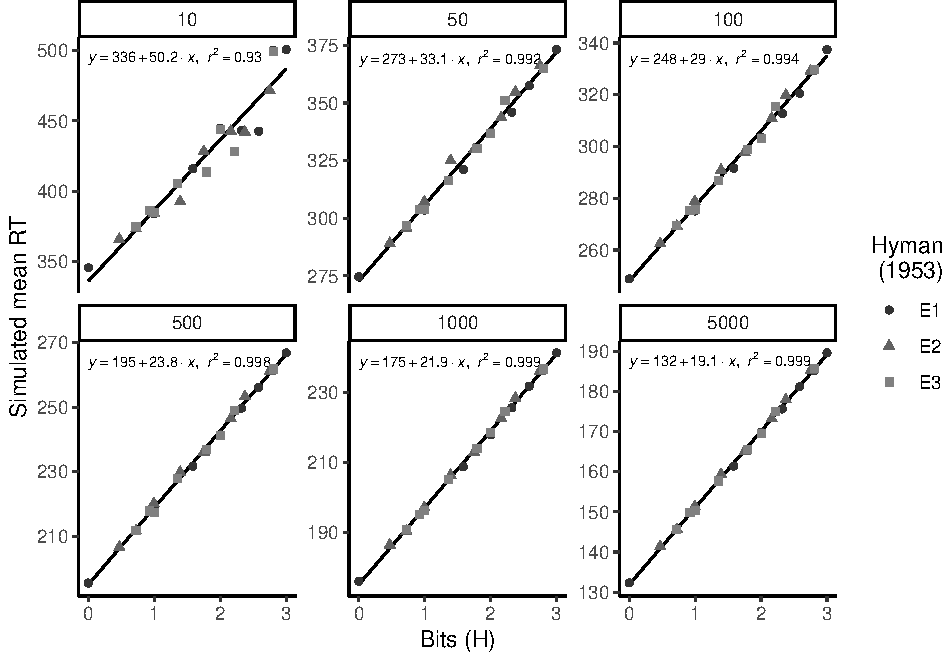
\includegraphics{Supplemental_materials_files/figure-latex/unnamed-chunk-1-1.pdf}

\hypertarget{references}{%
\section{References}\label{references}}

\begingroup
\setlength{\parindent}{-0.5in}
\setlength{\leftskip}{0.5in}

\hypertarget{refs}{}
\leavevmode\hypertarget{ref-behmer_crunching_2017}{}%
Behmer, L. P., \& Crump, M. J. C. (2017). Crunching big data with finger tips: How typists tune their performance towards the statistics of natural language. In M. N. Jones (Ed.), \emph{Big Data in Cognitive Science} (pp. 319--341).

\leavevmode\hypertarget{ref-Crump_Lai_Brosowsky_2018}{}%
Crump, M. J. C., Lai, W., \& Brosowsky, N. (2018, December). Instance theory predicts information theory: Episodic uncertainty as a determinant of keystroke dynamics. OSF. doi:\href{https://doi.org/10.17605/OSF.IO/BDNQR}{10.17605/OSF.IO/BDNQR}

\endgroup


\end{document}
